% Generated by documents/paper/figures/make_rq_appendix.py from the rq02_decision_accuracy README; do not edit.
\clearpage
\section{Decision accuracy across sizes}
\label{app:rq02_decision_accuracy}

\begin{rqfinding}
1. \textbf{A smaller fully trained model ranks the design variants close to a coin flip.} On benchmark accuracy alone, DA-size is 0.52, 0.54, 0.53, 0.55 and 0.57 from 90M to 1B (mean over 290--440 gated tasks). No proxy comes near $\tau$ = 0.90. (Figure~\ref{fig:app_rq02_decision_accuracy}.)

2. \textbf{The pooled line in the figure mixes two populations.} It reads 0.54, 0.58, 0.56, 0.55, 0.59 (90 \% jackknife $\pm$ 0.02--0.03), but its tasks include the bBPB twins at 175M and 1B (816 tasks) and at 350M (544) and none at 90M or 600M, so its zigzag is a change of tasks, not of size.

3. \textbf{Bits per byte ranks like the reference. Accuracy does not.} FineWeb2 BPB reads 0.96, 0.96, 0.92, 0.74, 0.92 (mean over 50 per-language tasks) and \texttt{bpb\_macro} 0.95--0.98.
\end{rqfinding}

\paragraph{Question.} Decision accuracy (DA) is the ground truth of the whole framework: the probability that a benchmark orders a pair of models the way an evaluation of larger models would (Heineman et al., 2025). Which benchmarks, in which languages, keep the ranking of the ladder's design variants across sizes (\textbf{DA-size}), across training (\textbf{DA-ckpt}), and early \emph{and} small at once (\textbf{DA-goal})?

\paragraph{Setup.} Seed-1904 runs of every language setting, ladder and data build, 90M--1.7B. DA-size is the share of design pairs that the final checkpoint of a proxy orders in the same way as the final checkpoint of the 1.7B reference. Every task is above chance at the proxy and at 1.7B. A pair may differ on any number of design axes.

\begin{figure}[h]
\centering
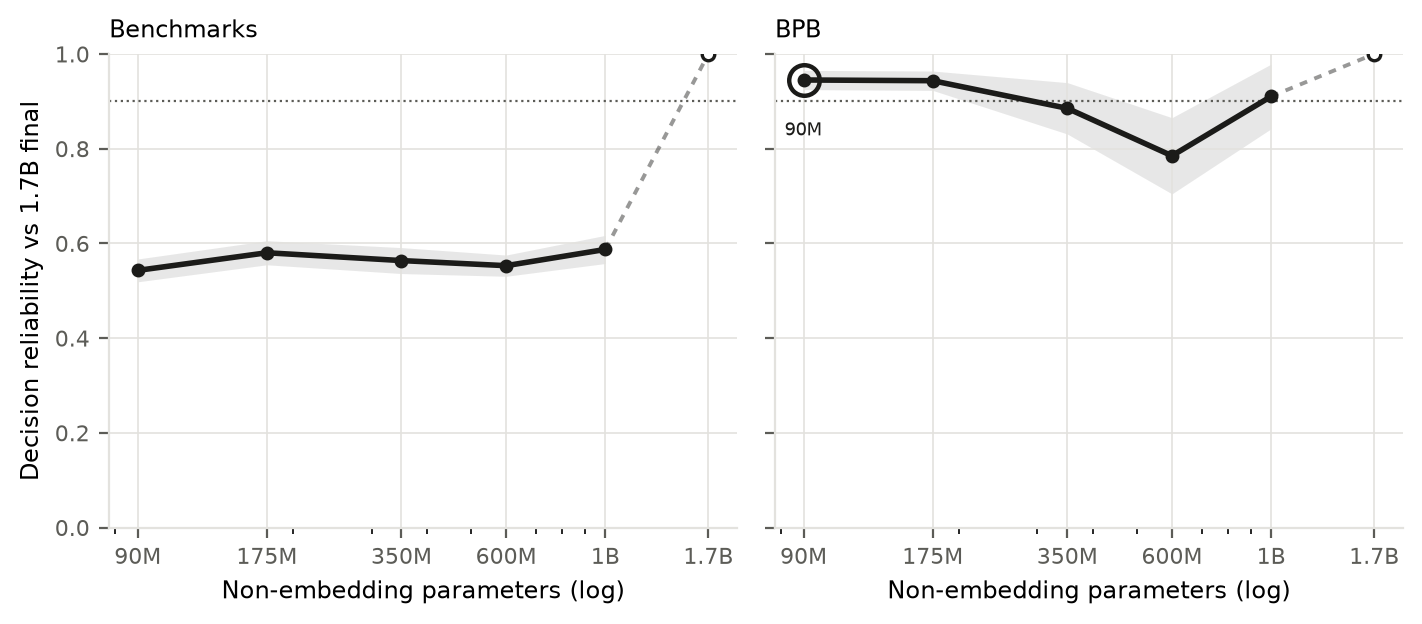
\includegraphics[width=\textwidth]{figures/app_decision_accuracy.png}
% source: src/signal-and-noise/analysis/rq02_decision_accuracy/pretraining/predictivity/scale_convergence_da_size_multi_axes_paper.png
\caption{Scale convergence, overall.}
\label{fig:app_rq02_decision_accuracy}
\end{figure}

\begin{figure}[p]
\centering
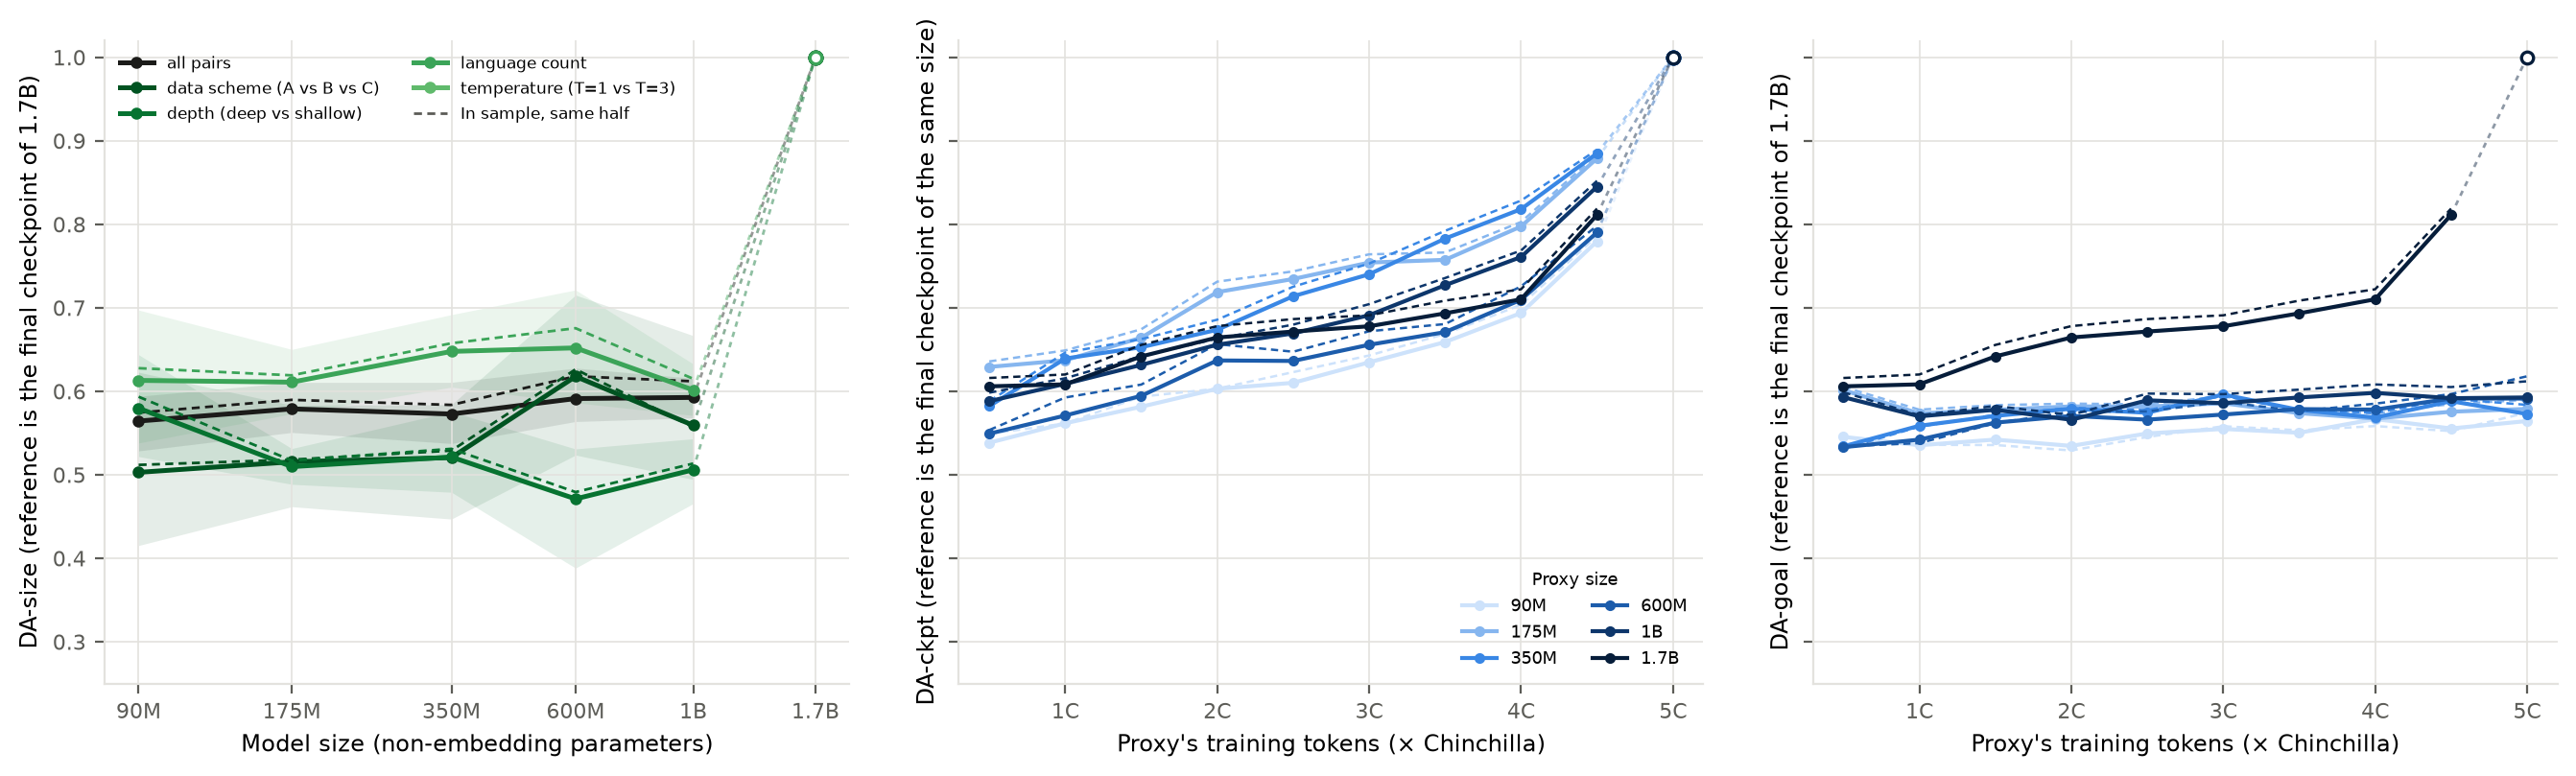
\includegraphics[width=\textwidth,height=0.9\textheight,keepaspectratio]{figures/app_rq2_crossfit.png}
% source: src/signal-and-noise/analysis/rq02_decision_accuracy/pretraining/predictivity/rq2_da_all_above_66_either_crossfit_transformation_mono_axis.png
\caption{Figure~\ref{fig:rq2} with the reliable tasks chosen out of sample. The verdict (DA above 0.66 on the size or the checkpoint axis) is decided on one half of the design pairs and the panels are read on the other half, over 20 random splits stratified by the axes a pair moves, in both directions (solid, with the 5--95\% range over splits). The dashed lines choose and read the tasks on the same half, so the gap between the two is the selection effect alone. Out of sample, DA-size over every single-axis pair changes by up to $-$0.03 (at 600M). Lines with too few pairs per half are not drawn.}
\label{fig:app_rq2_crossfit}
\end{figure}

\begin{figure}[p]
\centering
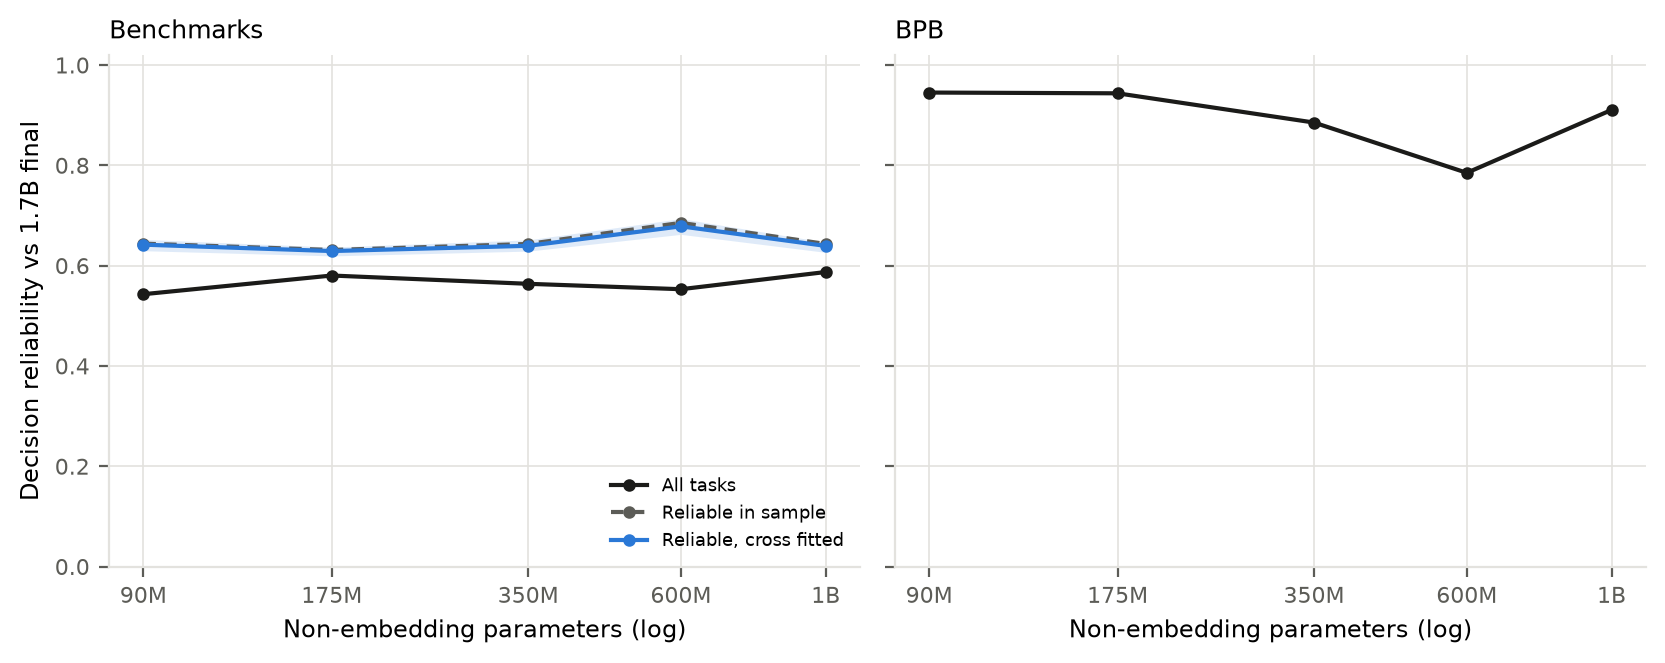
\includegraphics[width=\textwidth,height=0.9\textheight,keepaspectratio]{figures/app_decision_accuracy_crossfit.png}
% source: src/signal-and-noise/analysis/rq02_decision_accuracy/pretraining/predictivity/scale_convergence_da_size_above_66_either_crossfit_multi_axes_paper.png
\caption{Figure~\ref{fig:app_rq02_decision_accuracy} with the reliable benchmark tasks, chosen out of sample and in sample on the same half of the pairs (the same splits). The two readings differ by at most 0.01 on the multi-axis pairs.}
\label{fig:app_decision_accuracy_crossfit}
\end{figure}
